%!TEX root = ../../novoIndex.tex

%conceito, inspiração biológica
As \emph{Redes Neurais Artificiais} (RNAs) são um modelo de computação caracterizado por sistemas que, em algum nível, lembram a estrutura do cérebro humano. São sistemas paralelos e distribuídos, compostos por unidades de processamento simples, os \emph{neurônios artificiais}, que calculam funções matemáticas, normalmente não-lineares. Estes neurônios são dispostos em uma ou mais camadas e interligados por um grande número de conexões normalmente unidirecionais e comumente associadas a pesos, que armazenam o conhecimento representado no modelo e ponderam a entrada recebida por cada neurônio da rede. Os principais atrativos das RNAs envolvem a capacidade de capturar tendências a partir de um conjunto de exemplos e dar respostas coerentes para dados não-conhecidos, ou seja, de generalizar a informação aprendida \cite{Teresa:Livro}.

\begin{figure}[hb!]
	\caption{Redes neurais biológicas.}
	\begin{subfigure}[hb]{0.5\linewidth}
		\caption{Neurônio biológico e seus componentes. Fonte: \protect\cite{neuronio_biologico}}
		\label{fig:neuronio_biologico}
		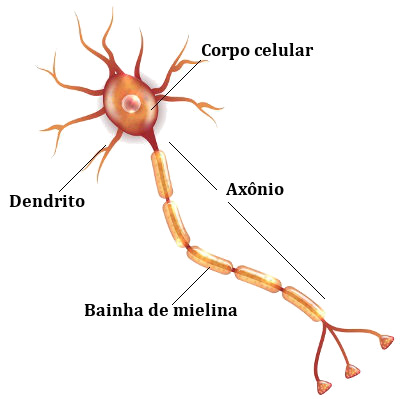
\includegraphics[width=0.7\linewidth]{img/neuronio}
	\end{subfigure}
	\begin{subfigure}[hb]{0.5\linewidth}
		\caption{Sinapse entre neurônios. Fonte: \protect\cite{sinapse}}
		\label{fig:redeneuralbiologica}
		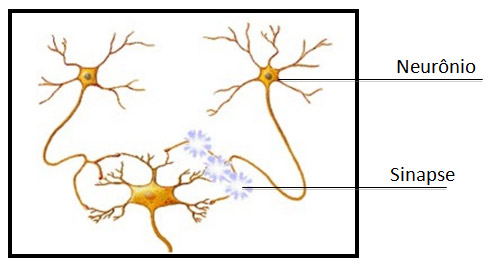
\includegraphics[width=\linewidth]{./img/redeneuralbiologica.jpg}
	\end{subfigure}%
\end{figure}

A motivação para a criação deste modelo vem do funcionamento do cérebro biológico, que é formado por neurônios interligados e que se comunicam entre si de modo contínuo e paralelo através de impulsos nervosos. Esta complexa rede neural biológica é capaz de reconhecer padrões e relacioná-los, produzir emoções, pensamentos, percepcção e cognição. Cada neurônio biológico é composto de um corpo, dendritos e um axônio, como ilustrado na Figura \ref{fig:neuronio_biologico}. Os dendritos são responsáveis pela recepção de impulsos nervosos vindos de outros neurônios; o corpo combina os sinais recebidos pelos dendritos e caso o resultado ultrapasse determinado limiar de excitação do neurônio, são gerados novos impulsos nervosos, que são transmitidos pelo axônio até os dendritos dos neurônios seguintes. Esta conexão unilateral entre neurônios biológicos, denominada sinapse, encontra-se ilustrada na Figura \ref{fig:redeneuralbiologica}.

Com base no modelo biológico, McCulloch e Pitts propuseram em \cite{mcculloch1943logical} um neurônio artificial. Como mostrado na Figura \ref{fig:neuronio}, o modelo de McCulloch e Pitts de neurônio artificial contém $n$ terminais de entrada, denotados por $x = x_1, \ldots, x_n$, e um terminal de saída $y$. Esta organização faz uma alusão aos dendritos, corpo celular e axônio de um neurônio biológico.

\begin{figure}[!ht]
	\centering
	\caption{Representação de um neurônio artificial. Fonte: \cite{neuronio:perceptron}}
	\label{fig:neuronio}
	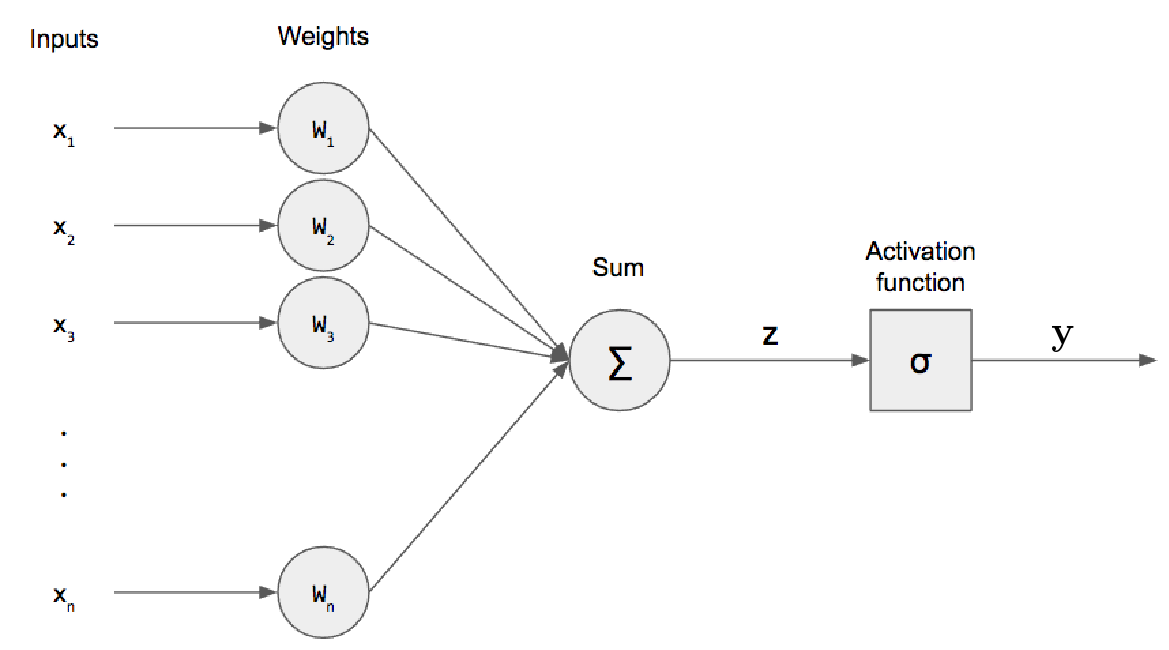
\includegraphics[width=0.7\textwidth]{img/perceptron.png}
\end{figure}
A saída $y$ é o resultado do mapeamento da função de ativação $\sigma$, conforme expresso na Equação \ref{eq:funcao_neuronio}, aplicada à soma ponderada do vetor de entrada $x$ pelo conjunto de pesos $w = w_1, \ldots, w_n$. No caso de um neurônio mais simples, como o de McCulloch e Pitts, a ativação do neurônio é obtida através da aplicação de uma função degrau deslocada, a depender da comparação da entrada com um limiar de ativação $\theta$, conforme Equação \ref{eq:ativacao_limiar} \cite{mcculloch1943logical}.
\begin{eqnarray}
	y &=& \sigma\left( z\right),\label{eq:funcao_neuronio}\\
	z &=& \sum_{i=1}^n x_i w_i\\
	\sigma(z) &=& \begin{cases}
		1, & \text{se } z \geq \theta\label{eq:ativacao_limiar}\\
		0, & \text{caso contrário.}
	\end{cases}
\end{eqnarray}
Considerando desenvolvimentos posteriores, sabe-se atualmente que a escolha da função de ativação $\sigma$ das camadas ocultas e da camada de saída deve considerar funções contínuas e deriváveis \cite{hornik1991approximation}, em que comumente são optadas pelas funções apresentadas na Tabela  \ref{tab:ativacoes}.

 %!TEX root = ../sbc-template.tex

\begin{table}[ht]
	\scalefont{0.8}
	\centering
	\caption{Funçoes de ativação mais populares. ---melhorar legenda}
	\label{tab:ativacoes}
	\begin{tabular}{l l p{6.5cm} l}
		\toprule
		Nome 			 		& Gráfico & Equação & Intervalo\\
		\midrule
		Identidade ou Linear		&
		 	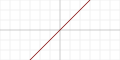
\includegraphics[width=0.1\textwidth]{img/identidade.png}
			&
			$
				\begin{aligned}
					g(z) = z
				\end{aligned}
			$
			& $(-\infty, + \infty) $\\
		\hline
		Tangente Hiperbólica		&
			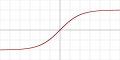
\includegraphics[width=0.1\textwidth]{img/tanh.png}
			&
			$
				\begin{aligned}
					g(z) = tanh(z) =\frac{(e^z - e^{-z})}{(e^z + e^{-z})}
				\end{aligned}
			$
			 & $(-1,1)$\\
		\hline
		Sigmoide ou Logística		&
			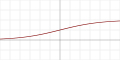
\includegraphics[width=0.1\textwidth]{img/sigmoid.png}
			&
			$
				\begin{aligned}
					g(z) = \sigma(z) = \frac{1}{1+e^{-x}}
				\end{aligned}
			$
			& $ (0,1) $\\
		\hline
		Unidade Linear Retificada	&
			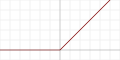
\includegraphics[width=0.1\textwidth]{img/relu.png}
			&
			$
				\begin{aligned}
					g(z) = max(0,z)
				\end{aligned}
			$
			& $ [0, \infty) $\\
		\hline
		Softmax					&
			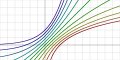
\includegraphics[width=0.1\textwidth]{img/softmax.png}
			&
			$
				\begin{aligned}
					g(\alpha, z) =
						\begin{cases}
							-\frac{ln(1-\alpha(z+\alpha))}{\alpha}, & \text{se } \alpha < 0\\
							z, & \text{se } \alpha = 0 \\
							\frac{e^{\alpha z} -1}{\alpha} + \alpha, & \text{se } \alpha > 0
						\end{cases}
				\end{aligned}
			$
			& $(-\infty, \infty)$\\
		\bottomrule
	\end{tabular}
\end{table}


Em 1958, Frank Rosenblatt desenvolveu o neurônio \emph{Perceptron} \cite{rosenblatt1958perceptron}, que mais tarde seria empregado como a unidade de processamento das RNA e de outros modelos de ML, a exemplo das máquinas de vetores de suporte. O Perceptron de Rosenblatt agregou ao neurônio de McCulloch e Pitts conceitos cruciais para a caracterização das RNAs como são conhecidas hoje, como a não obrigatoriedade de igualdade dos pesos e limiares de ativação, a possibilidade de os pesos serem positivos ou negativos, a diversidade de funções de ativação, entre outros. Além desta caracterização, uma contribuição relevante deste trabalho contempla a proposição de um algoritmo de aprendizado que permite a adaptação dos pesos de uma RNA através da otimização do desempenho da rede. Isto atribuiu ao modelo Perceptron a capacidade de aprender tarefas que contenham dados linearmente separáveis \cite{Teresa:Livro}.

Na ocasião de sua proposição, o modelo Perceptron apresentava algumas limitações, atribuídas principalmente à sua linearidade e simplicidade, características que possibilitam resolver apenas problemas linearmente separáveis \cite{Teresa:Livro}. Com o objetivo de tornar as RNAs aplicáveis em uma gama maior de problemas, os esforços de pesquisadores da área foram concentrados em aumentar e diversificar as técnicas aplicáveis a este modelo. Atualmente, as RNAs podem apresentar diversos tipos de arquitetura, ao variar-se parâmetros como o número de camadas, quantidade de neurônios em cada camada, os tipos de conexões entre neurônios e topologia de rede. Alguns exemplos de arquiteturas podem ser encontrados na Figura \ref{fig:popular_archs}.

\begin{figure}[!ht]
	\caption{Arquiteturas populares de RNAs. Fonte: \cite{rnas_tipos}}
	\label{fig:popular_archs}

	\begin{subfigure}[h]{0.15\linewidth}
		\caption{Perceptron de Camada Única}
		\label{fig:slp}
		\centering
		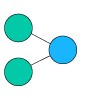
\includegraphics[width=0.6\linewidth]{img/pop_arch/single_layer_perceptron.jpg}
	\end{subfigure}
	\hspace{0.1cm}
	\begin{subfigure}[h]{0.15\linewidth}
		\caption{Radial Basis Network -- RBN}
		\label{fig:rbm}
		\centering
		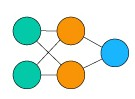
\includegraphics[width=0.9\linewidth]{img/pop_arch/radial_basis_network.jpg}
	\end{subfigure}
	\hspace{0.1cm}
	\begin{subfigure}[h]{0.3\linewidth}
		\caption{Multi Layer Perceptron -- MLP}
		\label{fig:mlp}
		\centering
		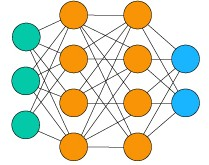
\includegraphics[width=0.75\linewidth]{img/pop_arch/mlp.jpg}
	\end{subfigure}
	\hspace{0.1cm}
	\begin{subfigure}[h]{0.3\linewidth}
		\centering
		\caption{Recurrent Neural Network -- RNN}
		\label{fig:rnn}
		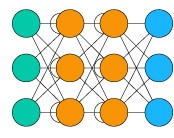
\includegraphics[width=0.6\linewidth]{img/pop_arch/rnn.jpg}
	\end{subfigure}\\

	\begin{subfigure}[h]{0.3\linewidth}
		\centering
		\caption{Long Short-Time Memory RNNs}
		\label{fig:lstm}
		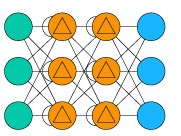
\includegraphics[width=0.6\linewidth]{img/pop_arch/lstm.jpg}
	\end{subfigure}
	\hspace{0.5cm}
	\begin{subfigure}[h]{0.3\linewidth}
		\centering
		\caption{Hopfield Network}
		\label{fig:hopfield}
		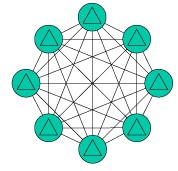
\includegraphics[width=0.6\linewidth]{img/pop_arch/hopfield.jpg}
	\end{subfigure}
	\hspace{0.5cm}
	\begin{subfigure}[h]{0.3\linewidth}
		\centering
		\caption{Boltzmann Machine}
		\label{fig:boltzmann}
		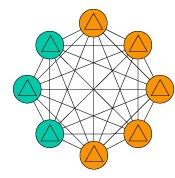
\includegraphics[width=0.6\linewidth]{img/pop_arch/boltzmann.jpg}
	\end{subfigure}
\end{figure}

\begin{table}[H]
	\centering
	\caption{Legenda das unidades presentes nas redes neurais da Figura \ref{fig:popular_archs}.}
	\label{tab:legenda_unidades}
		\begin{tabular}{l l}
			\toprule
			Imagem 			 		& Unidade\\
			\midrule
			\Centerstack{
\includegraphics[width=0.03\textwidth]{img/pop_arch/entrada.jpg}} & Entrada \\
			\hline
			\Centerstack{
\includegraphics[width=0.03\textwidth]{img/pop_arch/saida.jpg}} & Saída \\
			\hline
			\Centerstack{
\includegraphics[width=0.03\textwidth]{img/pop_arch/oculta.jpg}} & Oculta \\
			\hline
			\Centerstack{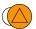
\includegraphics[width=0.05\textwidth]{img/pop_arch/feedback_memoria.jpg}} & Feedback com memória \\
			\hline
			\Centerstack{
\includegraphics[width=0.05\textwidth]{img/pop_arch/backfeed.jpg}} & Entrada retroalimentada \\
			\hline
			\Centerstack{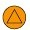
\includegraphics[width=0.05\textwidth]{img/pop_arch/probabilistica.jpg}} & Oculta probabilística \\
			\bottomrule
		\end{tabular}
\end{table}


% Desnecessário
%No que tange à conectividade, uma RNA pode ser classificada como parcialmente ou totalmente conectada. O primeiro caso ocorre quando apenas alguns dos neurônios da camada anterior estão conectados aos da camada posterior. A RNA é dita totalmente conectada se todos os neurônios da camada anterior estão conectados aos da camada posterior.

Quanto aos tipos de conexão possíveis entre os neurônios, tem-se que as RNAs podem ser do tipo \emph{feedforward} ou recorrente. As RNAs \emph{feedforward}, como a exemplificada na Figura \ref{fig:feedforward}, são comumente associadas a um grafo acíclico em que as saídas de uma camada servem de entrada à camada seguinte, e assim sucessivamente, até que seja produzida uma saída da rede. As RNAs recorrentes, tais como a rede exemplificada na Figura \ref{fig:recorrente}, contém conexões entre neurônios de modo a formar um grafo direcionado cíclico, o que permite que o modelo capture sequências de comportamentos organizados em séries temporais.

\begin{figure}[h!]
	\caption{Exemplos de RNA com diferentes tipos de conexões entre neurônios \cite{rna:feedback}.}
	\label{fig:rna_conectividade}
	\begin{subfigure}[h]{0.35\linewidth}
		\caption{Exemplo de RNA \emph{feedforward}.}
		\label{fig:feedforward}
		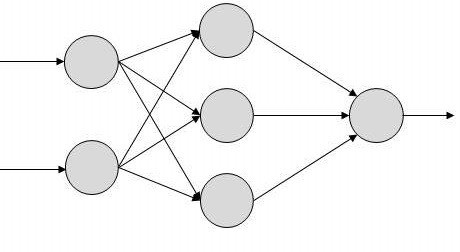
\includegraphics[width=\linewidth]{img/feedforward.jpg}
	\end{subfigure}
	\hfill
	\begin{subfigure}[h]{0.35\linewidth}
		\caption{Exemplo de RNA recorrente.}
		\label{fig:recorrente}
		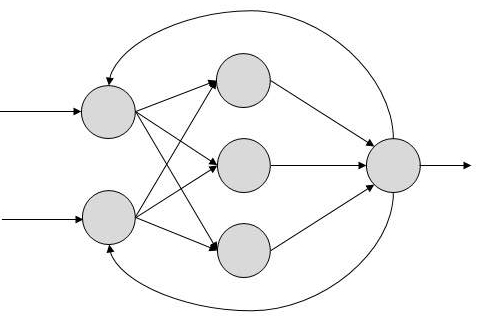
\includegraphics[width=\linewidth]{img/recorrente2}
	\end{subfigure}%
\end{figure}

Um dos parâmetros relacionados à arquitetura de uma RNA é a quantidade de camadas ocultas. Pode-se ter redes de camada única, compostas por um neurônio que conecta todos os parâmetros de entrada às saídas do modelo, a exemplo das redes Perceptron. Há também as redes de múltiplas camadas, que consistem de mais de um neurônio entre entrada e saída da rede, como retratado na Figura \ref{fig:mlp}. Redes com múltiplas camadas, as chamadas Redes Neurais \emph{Feedforward Multilayer Perceptron} (MLP), são capazes de aproximar diversas funções. Quando a Equação \ref{eq:funcao_neuronio} é aplicada a uma camada oculta $c$, de modo que a entrada da função nesta camada seja a saída da camada anterior $c-1$, o resultado $a^{c}$ é construído como mostrado na Equação \ref{eq:funcao_neuronio_camadas} e chamado de mapa de características ou \emph{feature map}. Para uma RNA com profundidade $C$, a saída prevista $\hat{y}$
é dada pelo mapa de característas $a^C$ \cite{hornik1991approximation,Teresa:Livro}.

\begin{gather}\label{eq:funcao_neuronio_camadas}
	z^c = \sum_{i=1}^n a_i^{c-1} w_i^c + b_i^c\\
	a^c = \sigma(z^c)
\end{gather}

Segundo o Teorema da Aproximação Universal definido por Hornik em 1991, se a ativação de uma rede neural MLP for uma função limitada e não-constante, então dada uma entrada $x$, a rede é capaz de aproximar qualquer função contínua, provida uma quantidade adequada de camadas ocultas. Esta característica atribui às redes neurais artificias o potencial de se tornarem máquinas de aprendizado universal \cite{hornik1991approximation}.

\begin{figure}[ht]
	\centering
	\caption{Rede Neural MLP com duas camadas ocultas.}
	\label{fig:mlp}
	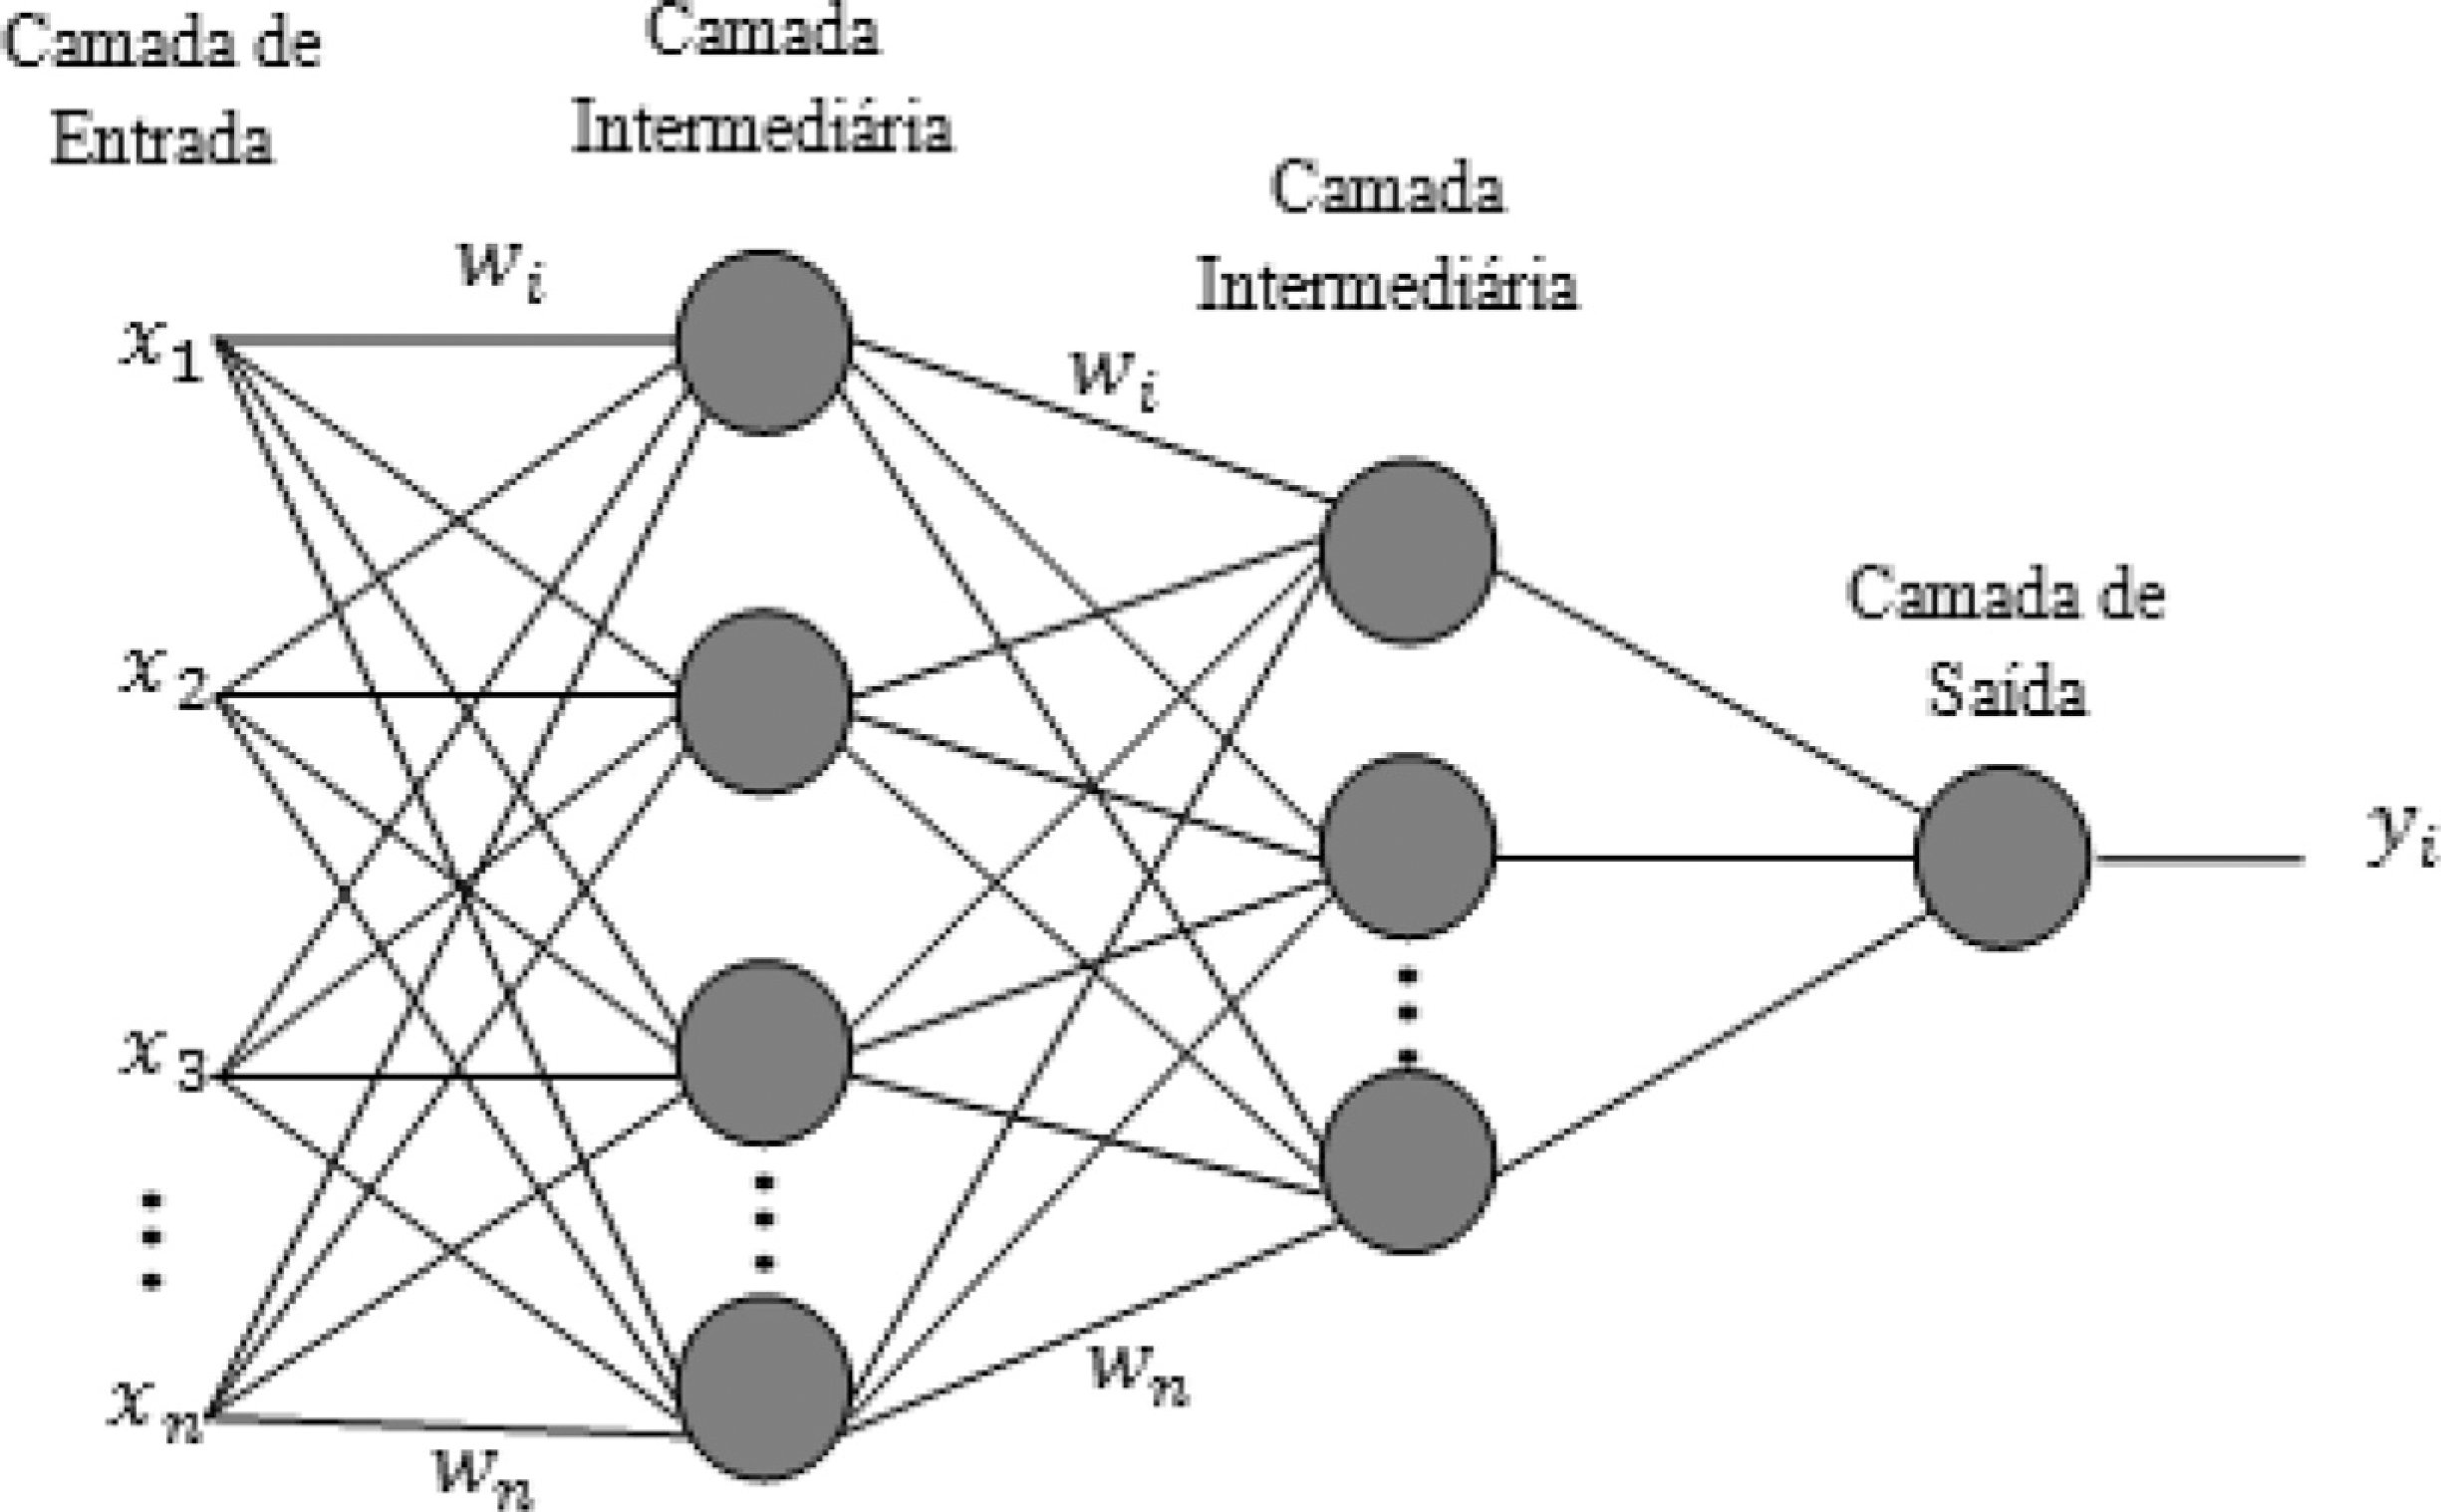
\includegraphics[width=0.6\textwidth]{img/mlprna.jpg}
\end{figure}

O objetivo das RNAs é aproximar funções que mapeiem entradas $x$ às suas respectivas saídas $y$. Para atingir este objetivo, é necessário minimizar a disparidade entre as saídas previstas $\hat{y}$ e as saídas desejadas $y$ através da atualização dos pesos $w$ e do \emph{bias} $b$ dos neurônios das camadas. A função que calcula tal disparidade é chamada \emph{função custo}, dada por $J$ e tida como a soma das funções de perda, $L(\hat{y}_i, y_i)$, entre cada saída esperada $y_i$ e obtida pela RNA $\hat{y}_i$, que é acumulada à medida que o modelo é apresentado a $m$ exemplos do evento que se deseja aprender. A função custo está representada na Equação \ref{eq:custo}, e a perda pode ser calculada de diversas maneiras, a depender do tipo de tarefa de aprendizado, função de ativação e algoritmo de otimização escolhidos.

\begin{equation}\label{eq:custo}
J = \frac{1}{m} \sum_{i=1}^{m} L(\hat{y}_{i}, y_{i}).
\end{equation}

No contexto de maximizar as previsões corretas de uma RNA, deve-se atualizar gradualmente os pesos e \emph{bias} do modelo de maneira a encontrar uma função que melhor represente o comportamento do fenômeno apresentado através dos dados, de maneira a minimizar a função custo para que haja a otimização do desempenho da RNA. Este procedimento é descrito pelo algoritmo de \emph{back-propagation}, que consiste em duas fases que se alternam: a fase \emph{forward} e a fase \emph{backwards} \cite{haykin2009neural}.

A fase \emph{forward}, também chamada \emph{forward propagation}, consiste na inferência das saídas da rede perante um conjunto de $m$ entradas, fornecidas à rede uma de cada vez. Neste processo, dada uma entrada $x_i$, a informação flui para frente  pela rede, isto é, as informações iniciais que são propagadas até as camadas ocultas, e de lá até que a saída $\hat{y}_i$ seja produzida. Ao final de uma fase \emph{forward}, a função custo $J$ é calculada. Modificações presentes na literatura também consideram algumas execuções da fase \emph{forward} para obtenção do custo médio nestas iterações. A representação da sequência de passos realizados nesta fase \emph{forward} está detalhada no Algoritmo \ref{alg:forward} \cite{haykin2009neural, goodfellow2016deep}.

\begin{algorithm}
	\caption{Fase \emph{forward}}\label{alg:forward}
	\Entrada{$i$-ésimo par de exemplos de entrada $x_i$ e saída $y_i$ do conjunto de treinamento}
	\Saida{Perda $L(\hat{y_i}, y_i)$}
	\Inicio{
	A entrada $x_i$ é apresentada à primeira camada da rede, como o primeiro vetor de características $a^0$ \\
	\Para {cada camada c=1,\ldots, C}{
		Calcular a saída da camada $a^c = \sigma^c(z^c)$, $z^c = w^c \times a^{c-1}$\\
	}
	Tomar como valor de saída do modelo a saída da última camada $\hat{y} = h^C$\\
	Calcular a perda $L(\hat{y_i}, y_i)$.
	}
\end{algorithm}

A fase \emph{backwards} é responsável por permitir que a informação referente à diferença entre os valores de saída obtidos $\hat{y}$ e os esperados $y$ calculada através da função custo na fase \emph{forward} flua para trás. Isto ocorre por meio da atualização dos pesos dos neurônios, a começar por aqueles localizados na camada de saída, passando pelas camadas ocultas, até atingir a camada de entrada. Ao percorrer este caminho contrário, para cada camada é calculado o gradiente $\delta$ da perda $L$ em função dos pesos e \emph{bias}, dado pela fórmula mostrada na Equação \ref{eq:gradiente}.

\begin{gather}\label{eq:gradiente}
	\delta_w = \nabla_{w} J = \left[
							\frac{\partial J}{\partial w_1}, \frac{\partial J}{\partial w_2}, \ldots, \frac{\partial J}{\partial w_n}
						\right]^T\\
	\delta_b = \nabla_{b} J = \left[
							\frac{\partial J}{\partial b_1}, \frac{\partial J}{\partial b_2}, \ldots, \frac{\partial J}{\partial b_n}
						\right]^T
\end{gather}

No contexto do cálculo, o gradiente indica o sentido e a direção para as quais se devem mover os valores dos pesos e \emph{bias} das camadas de maneira a se obter o maior incremento possível de perda. Considerando que o objetivo consiste na minimização \emph{gradual} dos parâmetros da rede na iteração $t+1$, o ajuste dos pesos e \emph{bias} dos neurônios na iteração $t$ é comumente realizado por meio do método gradiente descendente indicado na Equação \ref{eq:gradiente_descendente}, no qual o valor do gradiente $\delta$ é multiplicado por uma taxa de aprendizado $\eta$ e então subtraído dos valores de $w$ e $b$ \cite{haykin2009neural, goodfellow2016deep}.

\begin{gather}\label{eq:gradiente_descendente}
	w^c(t+1) = w(t) - \eta \nabla_{w^c} \\
	b^c(t+1) = b(t) - \eta \nabla_{b^c}
\end{gather}

A fase \emph{backwards}, denotada no Algoritmo \ref{alg:backpropagation}, lança mão de sequências de operações de regras da cadeia para calcular os gradientes. Inicialmente, o gradiente $\delta$ da função de ativação $\sigma$ da camada $l$ é obtido ao realizar o produto interno do gradiente calculado sob a função de custo da RNA pela derivada da função de saída $\sigma^c$. Esta combinação de derivações encadeadas é altamente eficiente, o que faz com que o o custo operacional da computação do gradiente seja $O(m)$, sendo $m$ o número de exemplos no conjunto de treinamento. Assim, o custo computacional cresce de maneira proporcional e linear à quantidade de exemplos presentes no conjunto de treinamento \cite{haykin2009neural, goodfellow2016deep}.

\begin{algorithm}
	\caption{Fase \emph{backwards}.}\label{alg:backpropagation}
	\Entrada{Custo $J$}
	\Saida{Gradientes dos parâmetros da RNA MLP atualizados}
	\Inicio{
		Calcular gradiente do custo, ou seja, da perda da camada de saída $\delta = \nabla_y J = \nabla_y L(\hat{y_i},y_i)$\\
		\Para {cada camada c=C,\ldots, 1}{
			Calcular o gradiente da camada $c$, dado por $\delta^c = \delta^{c-1} \cdot \sigma^c(z^c)$\\
			Atualizar variação em $w$, dada por $\nabla_{w^c} = \delta^c  a^{(c-1)}$\\
			Atualizar variação em $b$, dada por $\nabla_{b^c} = \delta^c$
		}
	}
\end{algorithm}

Além dos parâmetros $w$ e $b$, as RNAs MLP têm hiperparâmetros, responsáveis por controlar as mudança ocorridas nos parâmetros. Bengio define hiperparâmetros como variáveis cujos valores devem ser definidos antes que o algoritmo de treinamento se inicie. Alguns hiperparâmetros já discutidos neste texto são a taxa de aprendizado $\eta$, número de camadas ocultas, quantidade de neurônios e tipos de funções de ativação escolhidos para cada camada. O número de vezes que o conjunto de dados é apresentado ao modelo no treinamento, conhecido como número de épocas, também é um hiperparâmetro, assim como a quantidade de exemplos de treinamento apresentados à rede de uma só vez na fase \emph{forward}, chamado de \emph{batch size} \cite{bengio2012practical}.

Sumarizando os conceitos apresentados, o algoritmo para treinamento supervisionado de uma RNA MLP se dá como mostrado no Algoritmo \ref{alg:treinamento}.

\begin{algorithm}[h!]
	\caption{Algoritmo de treinamento de uma RNA  \cite{Teresa:Livro}.}\label{alg:treinamento}
	\Entrada{Conjuntos de exemplos e respectivos rótulos $(X,Y)$, rede neural a ser treinada, número de épocas $e$, taxa de aprendizado $\eta$ e \emph{batch size} $b$.}
	\Saida{Rede neural treinada.}
	\Inicio{
		Inicialização dos vetores de pesos $w$ e \emph{bias} $b$\\
		\Para {cada \emph{batch} = 1,\ldots, b do conjunto de dados}{
			Fase \emph{forward}: Calcular previsões $\hat{y}$ e custos $J$.\\
			Fase \emph{backwards}: Calcular gradientes dos pesos $\nabla_{w^c}$ e \emph{bias} $\nabla_{b^c}$\\
			Atualizar valores dos pesos e \emph{bias} a partir do gradiente descendente.
		}
	}
\end{algorithm}

Ao lidar com técnicas que visam acelerar ou potencializar o processo de aprendizado, o número de hiperparâmetros aumenta. Alguns exemplos destas técnicas incluem os algoritmos que realizam a otimização do gradiente descendente através da regularização dos pesos, como a Estimação Adaptativa do Momento, ou \emph{Adam} e o algoritmo de otimização da família dos métodos quase Newtonianos \emph{L-BFGS}. Outros hábitos comuns incluem a adoção de métodos de inicialização dos pesos que evitem o gradiente de convergir para pontos de sela, e de uma taxa de aprendizado que diminui conforme o número de épocas executadas aumenta para que o gradiente convirja para um ponto mínimo mais rapidamente \cite{goodfellow2016deep}.

As RNAs \emph{feedforward} MLP são amplamente utilizadas em aplicações de diversos domínios. Inicialmente, destacaram-se as aplicações voltadas para o mercado financeiro visando, por exemplo, otimizar estratégias de marketing. Aplicações posteriores consideraram a alocação de assentos em aviões, aprovação de empréstimo, controle de qualidade em processos industriais, dentre outros \cite{widrow1994neural}. O escopo de aplicações deste modelo continua a crescer nos dias atuais, especialmente diante do desenvolvimento de variantes, a exemplo das redes neurais convolucionais, com grande capacidade de detecção de padrões e pouco esforço de pré-processamento. Reconhecimento de caracteres e dígitos  \cite{lenet}, processamento de imagens médicas para reconhecimento de características associadas à doenças cardíacas \cite{oktay2018anatomically}, pulmonares \cite{mingchen2018holistic} e mamárias \cite{dubrovina2018mammography} são alguns exemplos de aplicações de vanguarda destes modelos compreendidos dentro da sub-área de \emph{Deep Learning}, que será caracterizada na seção a seguir.
